\newpage
\section{Method Signatures}
\genHeader
\hypertarget{static:methods vis}{}

To finish defining our types, lets define the \emph{signatures}\define{Operation Signature} of some operations that they'll eventually support.

\begin{stepbystep}

\item  Select \texttt{Partition} and either right-click to invoke the context-menu (\Cref{ea:add_operation})  and choose ``Features \&
Properties/Operations..'' or simply press \texttt{F10}.

\begin{figure}[htbp]
	\centering
  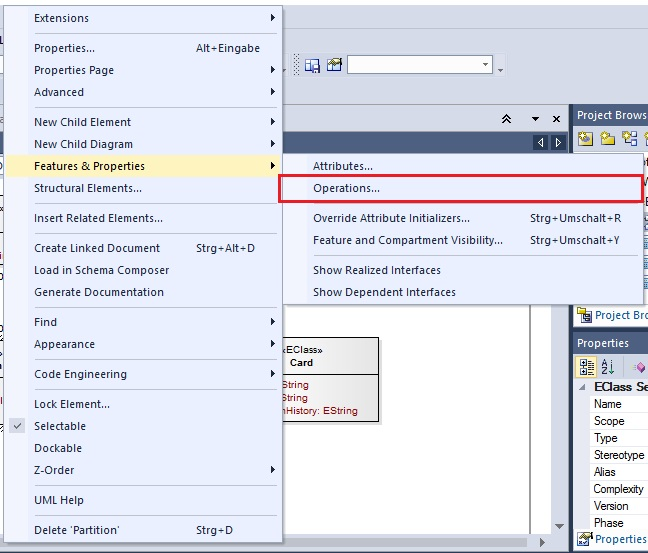
\includegraphics[width=0.8\textwidth]{../../org.moflon.doc.handbook.02_leitnersLearningBox/2_staticSemantics/4_creatingMethods/cmVisImages/ea_contextAddOperation}
	\caption{Add an operation}
	\label{ea:add_operation}
\end{figure}
\FloatBarrier

\item  In the dialogue that pops-up (\Cref{ea:operation_properties}), enter \texttt{empty} as the \texttt{Name} of the operation and \texttt{void} as the \texttt{Return Type}.

\vspace{0.5cm}

\item  In the same dialogue, click on \texttt{New Operation...} to add a second operation, \texttt{removeCard}, and edit the values as seen in 
\Cref{ea:operation_parameters}. Notice that the \texttt{Return Type} can be chosen by either the drop-down menu, or via direct typing. For types you've established in
the metamodel (e.g. \texttt{Card}) you have to use `\texttt{Select Type...}' from the drop-down menu.
\vspace{-.3cm}
\begin{quote}
{ \small
$\textbf{Very important:}$ Non-primitive types \emph{must} be chosen via `\texttt{Select Type...}' in the drop-down menu. It allows you to browse for the corresponding elements in
your project. Simply typing them won't work!
}
\end{quote}

\begin{figure}[htbp]
	\centering
  	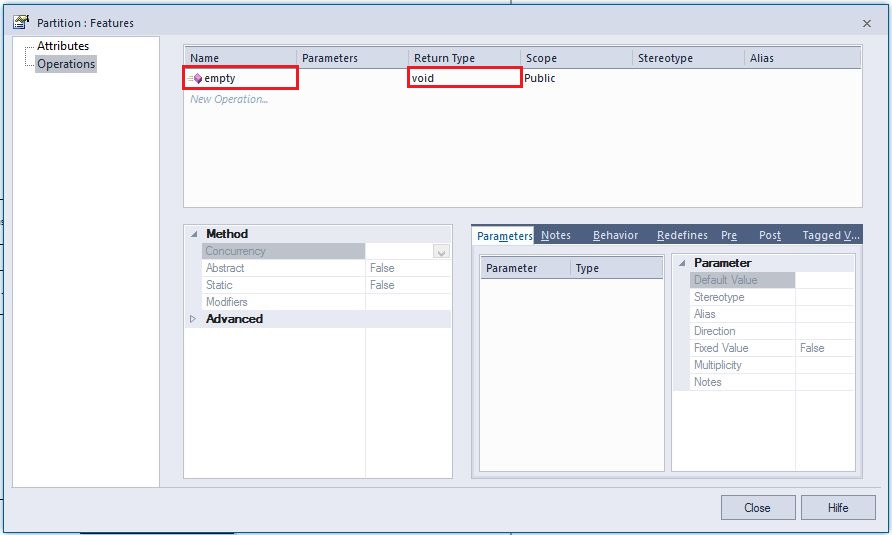
\includegraphics[width=\textwidth]{../../org.moflon.doc.handbook.02_leitnersLearningBox/2_staticSemantics/4_creatingMethods/cmVisImages/ea_operationEmpty}
	\caption{EClass properties editor}
	\label{ea:operation_properties}
\end{figure}


\item  Parameters can be added by selecting \texttt{Parameters} and
completing the dialouge (\Cref{ea:operation_parameters}). Please remember that you must also use either the drop-down menu, or direct typing to select the type or else validation
will fail.

\item  Repeat this process for the \texttt{check} operation (with the two parameters \texttt{card:Card, guess:EString}) that returns an \texttt{EBoolean}. 

\item  If you've done everything right, your dialogue should now contain three methods - \texttt{check}, \texttt{empty}, and
\texttt{removeCard} - each with the corresponding parameters and return types in \Cref{ea:operation_partition}.


\item  Add all operations analogously for \texttt{Box} and \texttt{Card} until your metamodel closely resembles
\Cref{ea:metamodel_complete}.\footnote{Please note that names of parameters may not be displayed by default in EA}

\item  To finish, export the metamodel for code generation in Eclipse, and examine the model once again. Each signature should have
appeared in their respective EClass.

\newpage

\vspace*{1cm}

\begin{figure}[htbp]
	\centering
  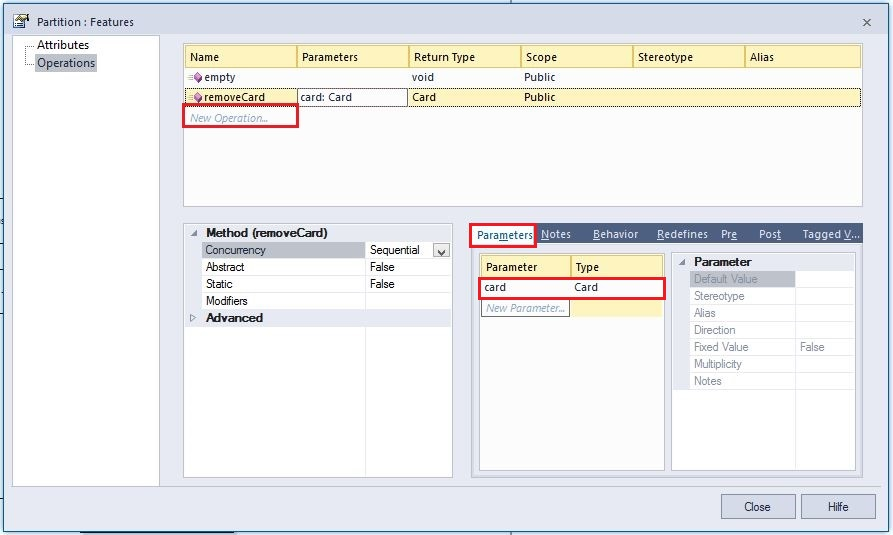
\includegraphics[width=\textwidth]{../../org.moflon.doc.handbook.02_leitnersLearningBox/2_staticSemantics/4_creatingMethods/cmVisImages/ea_operationRemoveCard}
	\caption{Parameters and return type}
	\label{ea:operation_parameters}
\end{figure}

\vspace{1cm}

\begin{figure}[h!]
	\centering
  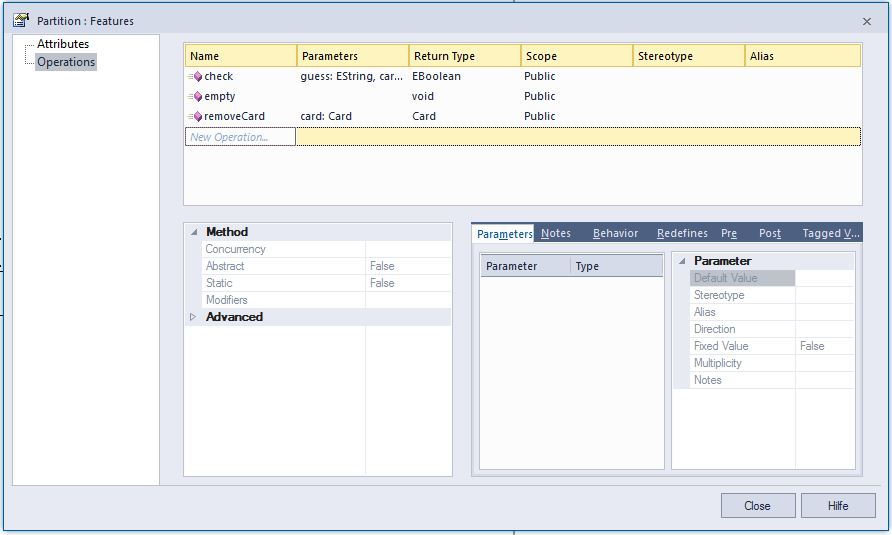
\includegraphics[width=\textwidth]{../../org.moflon.doc.handbook.02_leitnersLearningBox/2_staticSemantics/4_creatingMethods/cmVisImages/ea_operationCheck}
	\caption{All operations in \texttt{Partition}}
	\label{ea:operation_partition}
\end{figure}

\newpage


\begin{figure}[htbp]
	\centering
  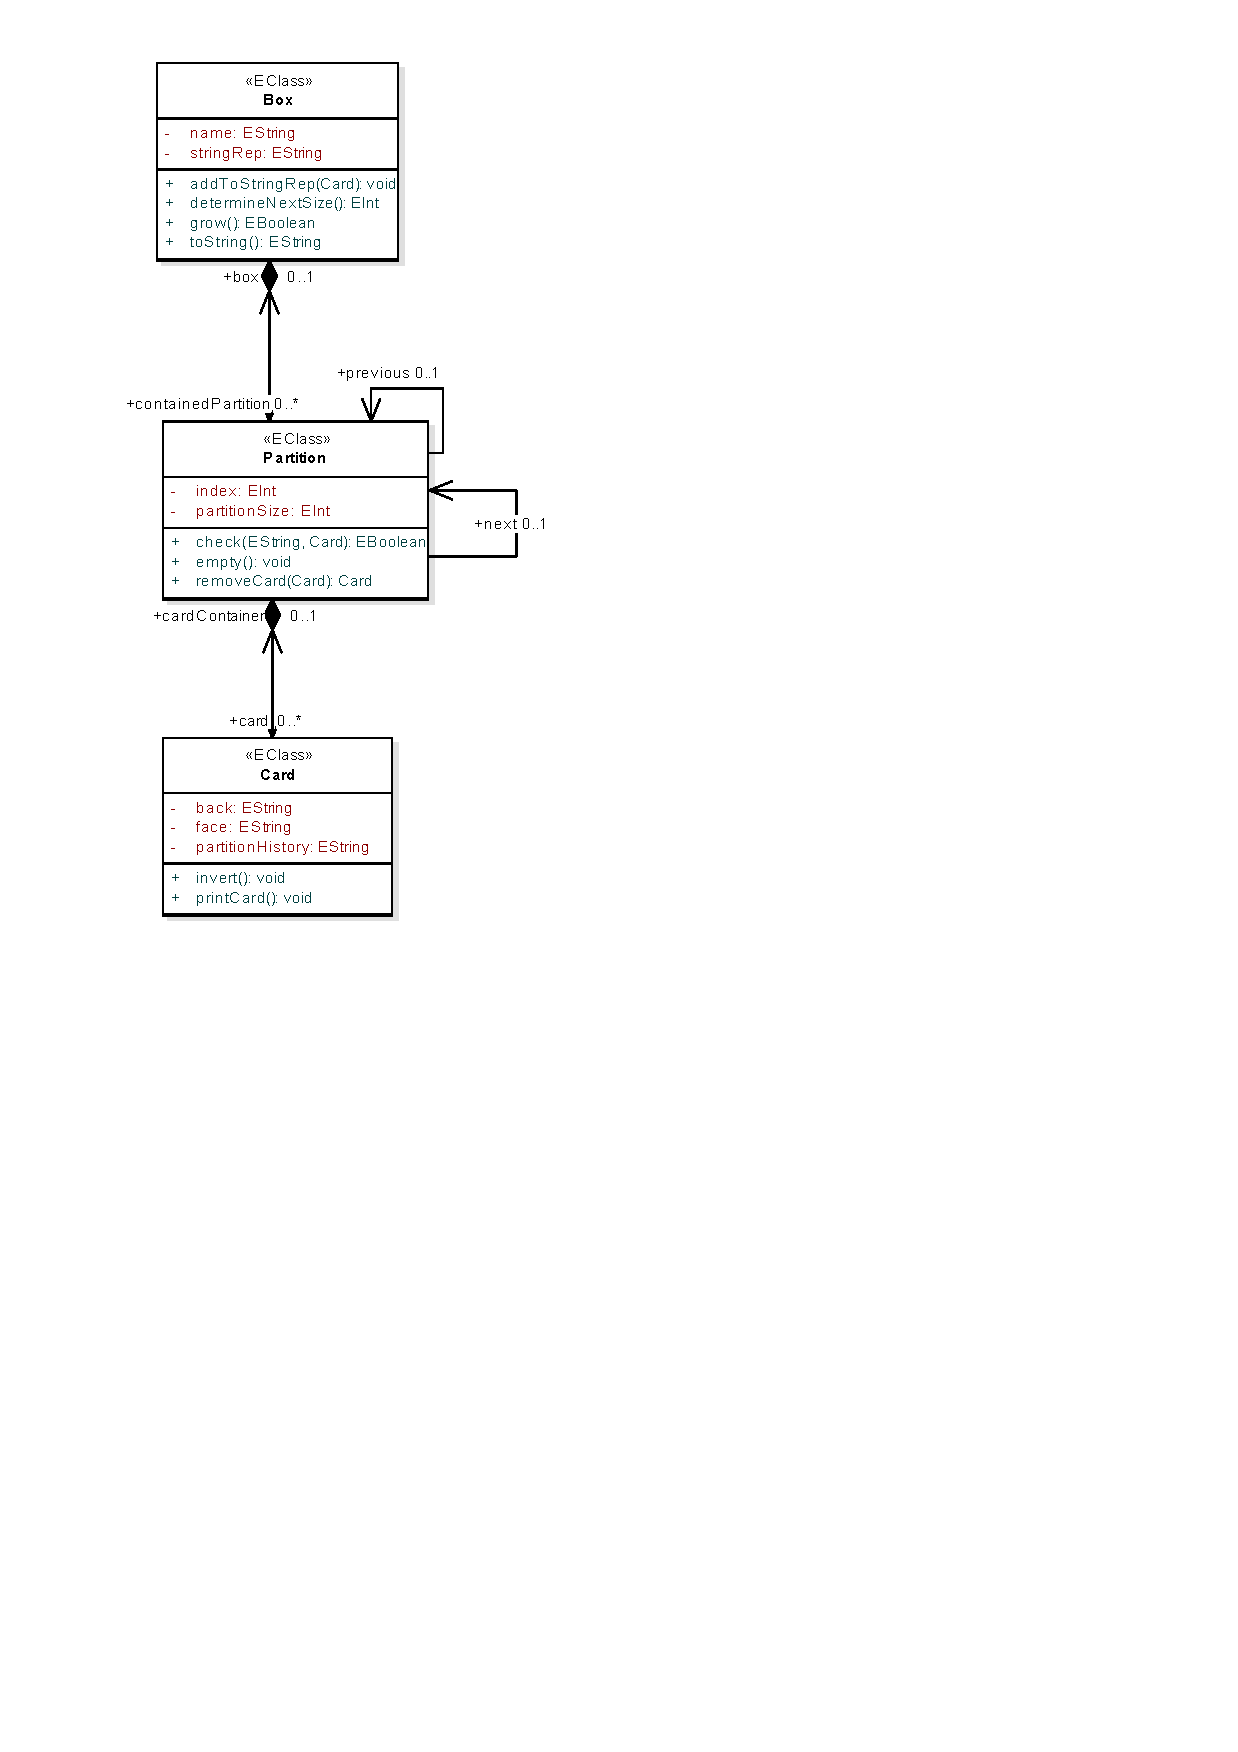
\includegraphics[width=0.6\textwidth]{../../org.moflon.doc.handbook.02_leitnersLearningBox/2_staticSemantics/4_creatingMethods/cmVisImages/ea_metamodelComplete}
\caption[Complete metamodel for our learning box.]{Complete metamodel for our learning box}
	\label{ea:metamodel_complete}
\end{figure}
\FloatBarrier

\end{stepbystep}

